% ==============================================================================
% SECAO 6 — SIMULACAO TEMPORAL E COMPARATIVO DE DESEMPENHO
% ==============================================================================
\section{SIMULAÇÃO TEMPORAL, SATURAÇÃO E COMPARATIVO DE DESEMPENHO}\label{sec:simulacao}

Com os projetos e as margens definidos na Seção~\ref{sec:projeto_comp}, as simulações de $0$ a $60\text{ s}$ confrontam o regime linear com a operação sujeita à saturação de capacidade e à perturbação de chegada.

\subsection{Resposta ao Degrau ($x_r = 300$), Evolução de $q(t)$ e Rejeição à Perturbação}\label{sec:resp_60s}
As simulações temporais no horizonte $t \in [0,\,60]\text{ s}$ avaliam o rastreamento da referência em degrau $x_r = 300\text{ eventos}$ aplicada em $t = 0$ (redução de $q(0)=600$ para $300\text{ eventos}$) e a rejeição à perturbação permanente de taxa de chegada $\Delta\lambda(t) = +100\,\mathbb{1}(t - 20)\text{ eventos/s}$ aplicada em $t = 20\text{ s}$. A Figura~\ref{fig:resposta_60s} compara as trajetórias de $x(t)$ e da fila real $q(t)$ tanto no modelo linear irrestrito quanto no modelo não linear com saturação $\mu_c,\mu \in [600,\,1400]\text{ eventos/s}$ e restrição física $q(t) \ge 0$.

Os resultados temporais distinguem as quatro estratégias de controle. O controlador P ($K_p = 0{,}369$) apresenta $t_r = 4{,}216\text{ s}$, $t_s = 13{,}752\text{ s}$ ($> 12\text{ s}$), $M_p = 10{,}55\%$ ($q_{\min} = 268{,}34$~eventos) e erro nulo antes da perturbação ($t < 20\text{ s}$); contudo, ao entrar a perturbação em $t=20\text{ s}$, a fila sobe até $q_{\max} = 619{,}16$~eventos e estabiliza com erro estacionário de $271{,}00$~eventos ($q_{ss} = 571{,}00$~eventos), perdendo quase toda a redução conquistada. O controlador PI ($K_p = 0{,}350,\; K_i = 0{,}030$) atinge $t_r = 3{,}614\text{ s}$, mas exibe sobressinal excessivo $M_p = 34{,}67\%$ ($q_{\min} = 195{,}99$~eventos) e acomodação lenta ($t_s = 19{,}578\text{ s}$); após $t = 20\text{ s}$, a fila eleva-se até $q_{\max} = 594{,}35$~eventos antes que a ação integral reconduza o sistema à referência $q_r = 300$~eventos (erro residual de $3{,}60$~eventos em $t=60\text{ s}$, convergindo a $0$ para $t \to \infty$, com tempo de recuperação $t_{s,\text{recup}} = 32{,}332\text{ s}$), coincidindo suas curvas linear e saturada por permanecer dentro de $[600,\,1400]$~eventos/s.

Por sua vez, o controlador PD ($K_p = 1{,}280,\; K_d = 1{,}560$, $\tau_f = 0{,}05\text{ s}$) apresenta transitório rápido na partida, com $t_r = 1{,}740\text{ s}$, $t_s = 6{,}018\text{ s}$ e $M_p = 4{,}70\%$ no modelo linear, ou $t_r = 3{,}096\text{ s}$, $t_s = 4{,}762\text{ s}$ e $M_p = 1{,}18\%$ com saturação e derivada na medição. Após $t = 20\text{ s}$, porém, estabiliza em $q_{ss} = 378{,}13$~eventos ($e_{ss,\text{dist}} = 78{,}13\text{ eventos} > 10$). Já entre os controladores PID ($\tau_f = 0{,}05\text{ s}$), o PID nominal ($\alpha = 0{,}15\text{ s}^{-1}$) cumpre todos os requisitos no caso linear ($t_r = 1{,}022\text{ s}$, $t_s = 10{,}440\text{ s}$, $M_p = 8{,}13\%$, $e_{ss,\text{dist}} = 0{,}15$~eventos em $60\text{ s}$), mas sob saturação física $[600,\,1400]$ com \textit{back-calculation} ($T_t=0{,}5\text{ s}$) e derivada na medição o sobressinal cai para $6{,}50\%$ enquanto $t_s$ eleva-se para $16{,}762\text{ s}$. Superando esse entrave, o PID ajustado ($\alpha = 0{,}40\text{ s}^{-1}$, $K_p=3{,}060,\,K_i=0{,}648,\,K_d=3{,}400$) com \textit{back-calculation} e derivada na medição alcança $t_r = 2{,}370\text{ s}$, $t_s = 10{,}744\text{ s}$ e $M_p = 6{,}98\%$, limitando o desvio máximo pós-perturbação a $q_{\max} = 343{,}84$~eventos com recuperação completa ($e_{ss,\text{dist}} = 0{,}00$~eventos) em $t_{s,\text{recup}} = 5{,}950\text{ s}$.

\begin{figure}[H]
    \centering
    \caption{Comparação temporal ($0$ a $60\text{ s}$) da redução da fila $x(t)$ e da fila real $q(t)$ para P, PI, PD e PID (à esquerda, regime linear; à direita, com saturação $[600,\,1400]\text{ eventos/s}$ e $q(t) \ge 0$), sob degrau $x_r = 300$ em $t=0$ e perturbação $\Delta\lambda = +100\text{ eventos/s}$ em $t=20\text{ s}$}
    \label{fig:resposta_60s}
    \IfFileExists{figuras/fig6_resposta_completa_60s.pdf}{%
        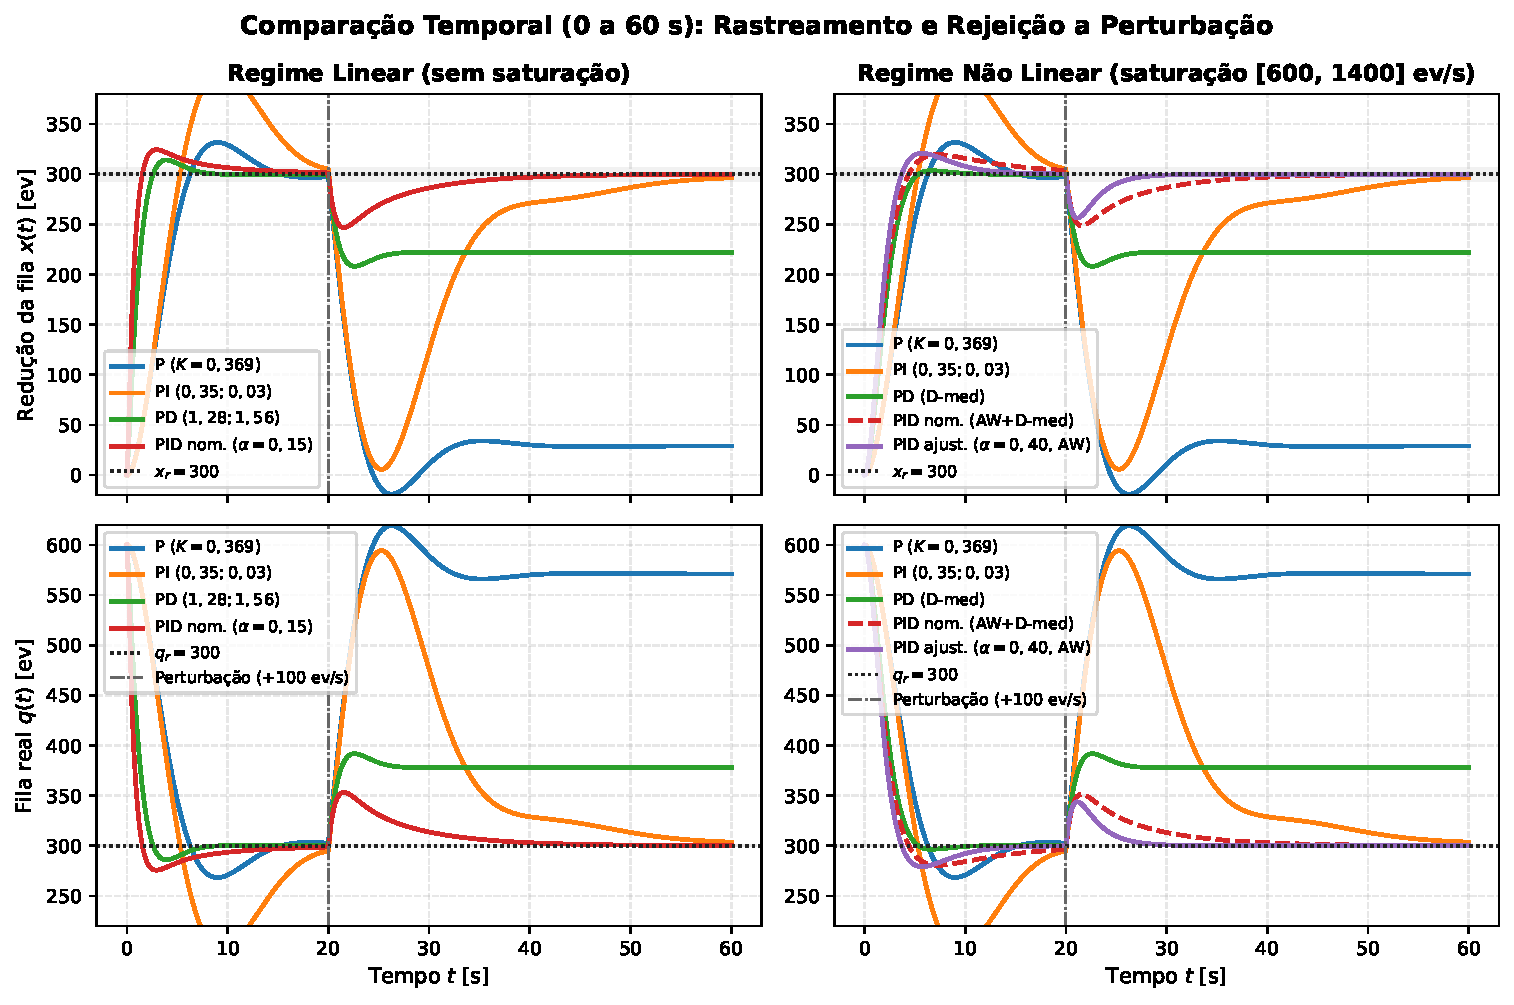
\includegraphics[width=0.78\textwidth]{figuras/fig6_resposta_completa_60s.pdf}%
    }{%
        \fbox{\parbox{0.80\textwidth}{\centering\vspace{1.0cm}\textit{[Aguardando \texttt{figuras/fig6\_resposta\_completa\_60s.pdf}]}\vspace{1.0cm}}}%
    }
    \fontefig{Fonte: Elaborada pelos autores com base nos resultados de simulação (2026).}
\end{figure}

\subsection{Avaliação da Capacidade Solicitada $\mu_c(t)$ e Efetiva $\mu(t)$ sob Saturação}\label{sec:cap_sat}
A Figura~\ref{fig:capacidade_sat} compara a capacidade solicitada $\mu_c(t)$ com a capacidade efetivamente entregue $\mu(t)$ e com os limites de $600$ e $1400\text{ eventos/s}$. Os controladores P e PI estável não atingem a saturação em nenhum instante ($t_{\text{sat}} = 0\text{ s}$), com picos de solicitação de $1117{,}77$ e $1143{,}18\text{ eventos/s}$, respectivamente. Essa folga, porém, é consequência dos ganhos moderados que tornam suas respostas lentas ou oscilatórias.

Nos controladores com ação derivativa, o perfil de $\mu_c(t)$ depende de onde a derivada é aplicada. Sobre o erro, o degrau $x_r = 300\text{ eventos}$ produz picos fisicamente irrealizáveis em $\mu_c(0^+)$: $10744\text{ eventos/s}$ no PD e $19048\text{ eventos/s}$ no PID nominal. Sobre a medição, o PD solicita no máximo $1384{,}00\text{ eventos/s}$ e não satura ($t_{\text{sat}} = 0\text{ s}$), o PID nominal limita-se a $1648{,}00\text{ eventos/s}$ e o PID ajustado chega a $1918{,}00\text{ eventos/s}$, permanecendo saturado por apenas $0{,}534\text{ s}$ no transitório inicial.

Em todos os casos, a capacidade efetiva permanece no intervalo operacional, porque a solicitação é ceifada em $[600,\,1400]\text{ eventos/s}$ antes de alimentar a dinâmica de primeira ordem de ganho unitário da infraestrutura. A resposta dessa dinâmica a uma entrada limitada fica contida nos mesmos limites. A constante de tempo $\tau = 2\text{ s}$ explica, além disso, por que os intervalos saturados, todos inferiores a $0{,}75\text{ s}$, quase não aparecem em $\mu(t)$: no PID ajustado, a capacidade efetiva atinge no máximo $1130{,}21\text{ eventos/s}$ e converge para $1100{,}00\text{ eventos/s}$ após $t = 20\text{ s}$, valor necessário para equilibrar a nova taxa de chegada.

\begin{figure}[H]
    \centering
    \caption{Capacidade solicitada $\mu_c(t)$ (painéis superiores) e capacidade efetiva $\mu(t)$ (painéis inferiores) ao longo de $60\text{ s}$ e detalhe dos primeiros $6\text{ s}$, comparando as solicitações aos limites físicos $[600,\,1400]\text{ eventos/s}$}
    \label{fig:capacidade_sat}
    \IfFileExists{figuras/fig7_capacidade_saturacao.pdf}{%
        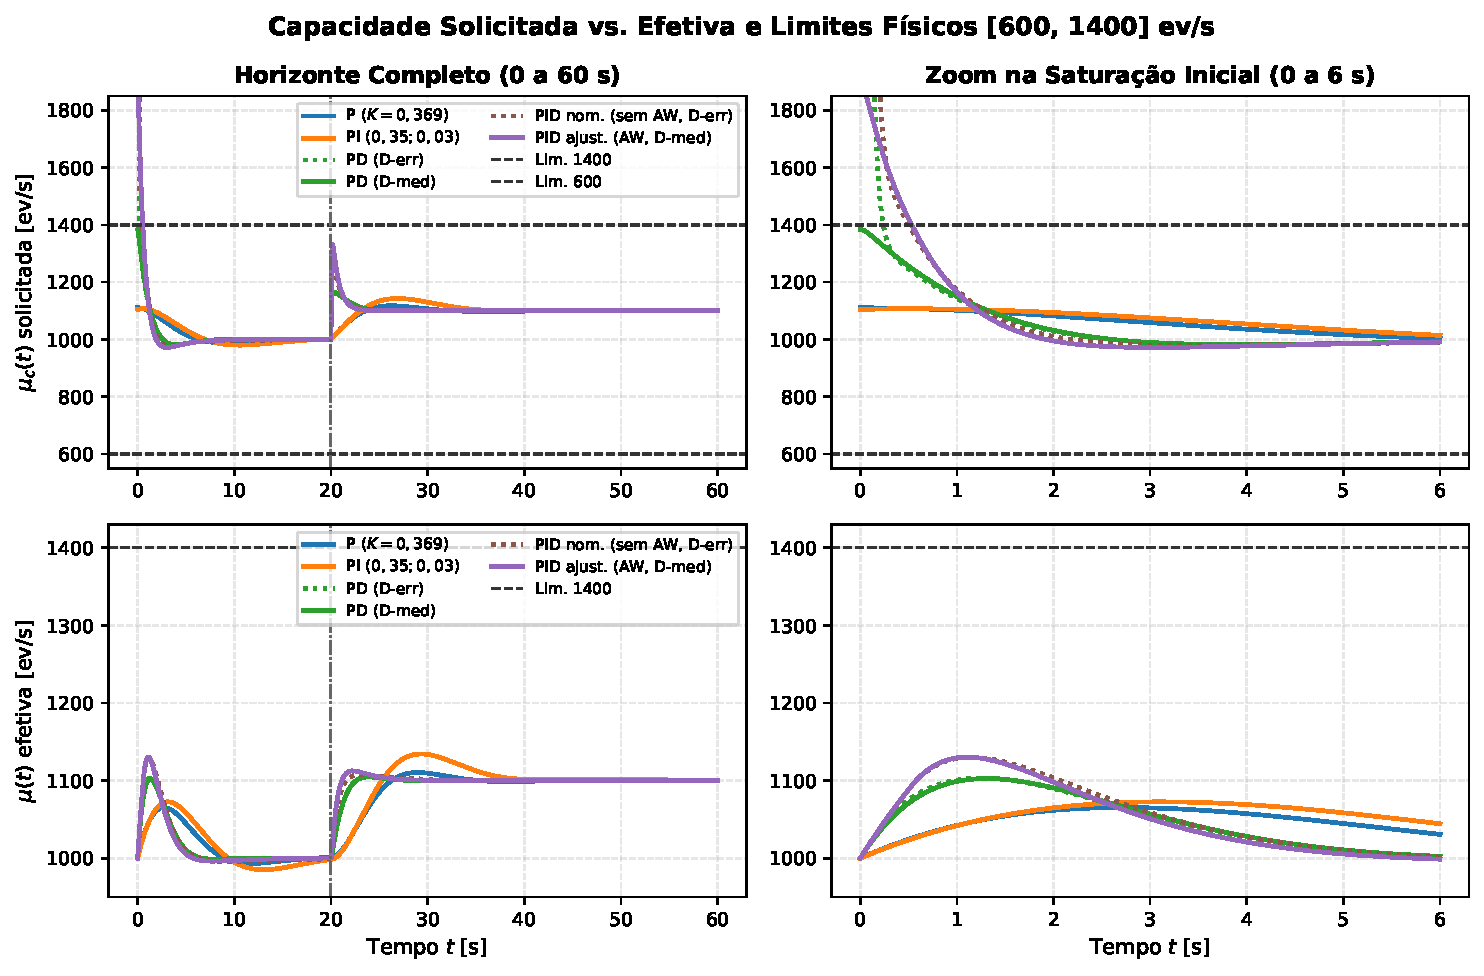
\includegraphics[width=0.78\textwidth]{figuras/fig7_capacidade_saturacao.pdf}%
    }{%
        \fbox{\parbox{0.80\textwidth}{\centering\vspace{1.0cm}\textit{[Aguardando \texttt{figuras/fig7\_capacidade\_saturacao.pdf}]}\vspace{1.0cm}}}%
    }
    \fontefig{Fonte: Elaborada pelos autores com base nos resultados de simulação (2026).}
\end{figure}

\subsection{Síntese Comparativa de Desempenho}\label{sec:tabela_comp}
A Tabela~\ref{tab:comparativo} consolida todos os indicadores quantitativos de desempenho estabelecidos na Seção~\ref{sec:requisitos} para as configurações analisadas (varredura do controlador P, PI estável e instável, PD linear e saturado, PID nominal linear e sob saturação, e PID ajustado sob saturação).

\begin{table}[H]
\centering
\caption{Comparativo consolidado de ganhos, estabilidade, métricas transitórias, erros estacionários, margens frequenciais e capacidade}
\label{tab:comparativo}
{\small\singlespacing
\resizebox{\textwidth}{!}{%
\begin{tabular}{llccccccccccc}
\toprule
\textbf{Controlador / Variante} & \textbf{Ganhos ($K_p;\, K_i;\, K_d$)} & \textbf{Estável} & $t_r$ (s) & $t_s$ (s) & $M_p$ (\%) & $e_{ss,\text{ref}}$ & $e_{ss,\text{dist}}$ & $\mathrm{GM}$ & $\mathrm{PM}$ ($^\circ$) & $\mu_{c,\max}$ & $\mu_{\max}$ & \textbf{Atende?} \\
\midrule
P ($K=0{,}080$) & $0{,}080;\; 0;\; 0$ & Sim & $23{,}120$ & $41{,}998$ & $0{,}00$ & $0{,}99^\dagger$ & $1226{,}57^\dagger$ & $\infty$ & $81{,}02$ & $1098{,}1$ & $1097{,}7$ & Não \\
P ($K=0{,}125$) & $0{,}125;\; 0;\; 0$ & Sim & $13{,}432$ & $23{,}336$ & $0{,}00$ & $0{,}00$ & $799{,}78^\dagger$ & $\infty$ & $76{,}35$ & $1100{,}0$ & $1100{,}0$ & Não \\
P ref. ($K=0{,}369$) & $0{,}369;\; 0;\; 0$ & Sim & $4{,}216$ & $13{,}752$ & $10{,}55$ & $0{,}00$ & $271{,}00$ & $\infty$ & $57{,}97$ & $1117{,}8$ & $1110{,}5$ & Não \\
P ($K=2{,}000$) & $2{,}000;\; 0;\; 0$ & Sim & $1{,}260$ & $14{,}118$ & $44{,}43$ & $0{,}00$ & $50{,}00$ & $\infty$ & $28{,}02$ & $1600{,}0$ & $1213{,}5$ & Não \\
\midrule
PI estável & $0{,}350;\; 0{,}030;\; 0$ & Sim & $3{,}614$ & $19{,}578$ & $34{,}67$ & $-0{,}13^\dagger$ & $3{,}60^\dagger$ & $\infty$ & $42{,}78$ & $1143{,}2$ & $1134{,}4$ & Não \\
PI instável (linear) & $0{,}500;\; 0{,}300;\; 0$ & \textbf{Não} & N/A & N/A & N/A & N/A & N/A & $\infty$ & $-5{,}21$ & $2042{,}9$ & $1752{,}5$ & Não \\
\midrule
PD linear ($\tau_f=0{,}05$) & $1{,}280;\; 0;\; 1{,}560$ & Sim & $1{,}740$ & $6{,}018$ & $4{,}70$ & $0{,}00$ & $78{,}13$ & $\infty$ & $75{,}33$ & $10744{,}0$ & $1228{,}4$ & Não \\
PD sat. + D-med & $1{,}280;\; 0;\; 1{,}560$ & Sim & $3{,}096$ & $4{,}762$ & $1{,}18$ & $0{,}00$ & $78{,}13$ & $\infty$ & $75{,}33$ & $1384{,}0$ & $1104{,}7$ & Não \\
\midrule
PID nom. linear ($\alpha=0{,}15$) & $2{,}160;\; 0{,}243;\; 2{,}900$ & Sim & $1{,}022$ & $10{,}440$ & $8{,}13$ & $0{,}00$ & $0{,}15^\dagger$ & $\infty$ & $77{,}67$ & $19048{,}0$ & $1397{,}0$ & \textbf{Sim} (lin.) \\
PID nom. sat. s/ AW & $2{,}160;\; 0{,}243;\; 2{,}900$ & Sim & $2{,}236$ & $21{,}680$ & $15{,}79$ & $-0{,}02^\dagger$ & $0{,}13^\dagger$ & $\infty$ & $77{,}67$ & $19048{,}0$ & $1130{,}1$ & Não \\
PID nom. sat. BC + D-med & $2{,}160;\; 0{,}243;\; 2{,}900$ & Sim & $2{,}802$ & $16{,}762$ & $6{,}50$ & $-0{,}01^\dagger$ & $0{,}14^\dagger$ & $\infty$ & $77{,}67$ & $1648{,}0$ & $1114{,}8$ & Não \\
\textbf{PID ajust. sat. BC + D-med} & $\mathbf{3{,}060;\; 0{,}648;\; 3{,}400}$ & \textbf{Sim} & $\mathbf{2{,}370}$ & $\mathbf{10{,}744}$ & $\mathbf{6{,}98}$ & $\mathbf{0{,}00}$ & $\mathbf{0{,}00}$ & $\boldsymbol{\infty}$ & $\mathbf{73{,}28}$ & $\mathbf{1918{,}0}$ & $\mathbf{1130{,}2}$ & \textbf{Sim (Todos)} \\
\bottomrule
\end{tabular}%
}}
\fontefig{$^\dagger$ Valor simulado em $t = 60\text{ s}$ (ensaio sem perturbação para $e_{ss,\text{ref}}$; ensaio completo para $e_{ss,\text{dist}}$, ainda em convergência para $0{,}00$ ou $100/K$). N/A: métrica não aplicável a sistema instável. BC: \textit{back-calculation} ($T_t=0{,}5\text{ s}$). Unidades: $e_{ss,\text{ref}}$ e $e_{ss,\text{dist}}$ em eventos; $\mu_{c,\max}$ e $\mu_{\max}$ em eventos/s; $\mathrm{GM}$ em dB.\\ Fonte: Elaborada pelos autores com base nos resultados de simulação (2026).}
\end{table}
